\chapter{Palabras acumuladas}
% Intro {{{
La búsqueda para cuantificar la influencia, ha llevado a contabilizar las
palabras que son nuevas en los distintos receptores y a partir de ellas ligar
contextos que sustenten la aparición de palabras.  Se ha puesto énfasis en el
conjunto de búsqueda, pero  el conjunto base  también tiene información sobre
las palabras que han migrado, además  abarca más años (160 comprendidos entre
1740 y 1900), por lo que su información es más basta en contenido. 

Para no repetir el proceso de contabilizar a los préstamos nuevos,  se propone
pensar que en el primer año del conjunto de búsqueda (1900),  el idioma
receptor ya contenía cierta cantidad de palabras que provenían de otros
orígenes\cpnote{A que te refieres con orígenes?},  de tal manera que ya forman parte de él, es decir estos préstamos
``conviven'' con las palabras propias de el receptor y son empleadas
indistintamente\cpnote{No entiendo lo que quieres decir en esta frase. 
Sugiero que la redactes mejor o me la expliques en persona.}. Así el conjunto
base proporcionará un sostén de aquellas palabras que han permeado en un idioma
y son utilizadas en los años del conjunto de búsqueda,  cabe decir que este
sostén crecerá conforme se localicen nuevas palabras\cpnote{acá tampoco entiendo}. 

Es necesario hacer una nueva definición para estos préstamos, dados un idioma  origen  \textit{A} y la lista para un año  de las palabras más comunes en el receptor \textit{B}, se definen como: 

\begin{description}
	\item[préstamos acumulados:] Son las palabras con origen \textit{A} que ya habían aparecido en alguna lista de \textit{B}, y para ese año lo volvieron a hacer.  \cpnote{Es decir que volvieron a aparecer, o que siguen estando? no me queda claro. En la frase despues, lo aclaras, pero siento que la definicion está deficiente. Igual porfa no quites la siguiente frase.}
\end{description}
\cpnote{No entiendo porque cambias el formato. Sugiero seguir con el parrafo como va. De hecho veo que en el capitulo 3, al principio tienes un formato similar. Cambia ambos e integralos en el texto. En la seccion 2.2 me gusta como tienes esas primeras 4 definiciones. Las
primeras dos, integradas en una frase, y las siguientes dos, como parte de una frase dentro de items. }

La diferencia entre los nuevos y los acumulados es que un préstamo será nuevo
sólo en el año de aparición, posteriormente se convertirá en acumulado. El
objetivo  de trabajar con los acumulados es ver cómo se comportan las palabras
que ya han migrado a un receptor y si hay tendencias donde su empleo se vea
alterado\cpnote{Que quieres decir con esa ultima frase? Que comportamiento? No se
que podemos decir con los datos que tenemos}.  

En el capitulo anterior, la atención se enfocaba en la cantidad de palabras,
nunca se trato con su frecuencia o su rango, ahora se utilizarán estas
propiedades  para llegar a una cantidad que cuantifique la influencia. Si se
tienen la lista de las cinco mil palabras más usadas  de \textit{B}, y se
distinguen en ella los préstamos acumulados con origen \textit{A}, entonces:
\cpnote{Oye, no me queda claro que estas usando el doble punto de manera
correcta. Puedes porfa verificar en un manual de ortografía ygramática que lo
estas haciendo bien?}


\begin{enumerate}
	
	\item En un año determinado del idioma \textit{B}, se sumarán las
	frecuencias $f_{k}$ de las cinco mil palabras más usadas.  Esta
	cantidad se llamará \textbf{frecuencia total} $f_{t}$ y es distinta año
	con año. 
	\begin{equation}
	\label{ec.ftot}
	f_{t} = \sum_{k=1}^{5000} f_{k} \,\,\,\,\,\,\,\,\, k = rango\,\, de \,\,cada \,\,palabra
	\end{equation}
	\cpnote{el texto en una ecuaccion se pone de otra manera. Además, no
	tienes necesitad de ponerlo ahi, mejor en lo que sigue. Ademas, tu
	notacion esta chafa. Si tenemos $f_5$ es a tiempo 5 o para el rango 5?
	Dale una iterada a todo este capitulo. Veo que 
	no esta tan pulida como otros capitulos. }
	\item Como se conocen los rangos $j$,  que ocupan los préstamos \textit{A} en la lista de \textit{B}, se procede a sumar sólo las frecuencias asociadas a estas palabras. Esta cantidad será la \textbf{frecuencia de préstamo} $f_{p}$,  siempre será menor que la frecuencia total.
	
	\begin{equation}
	\label{ec.fpres}
	f_{p} = \sum_{j} f_{j} \,\,\,\,\,\,\,\,\, j = rango\,\, de \,\,cada \,\,pr\acute{e}stamo\,\,acumulado
	\end{equation}
	
	
	\item  Se divide la frecuencia de préstamo entre la frecuencia total , esta cantidad se llamará  \textbf{Uso} $U$ y es la porción que representa \textit{A} en \textit{B} en teŕminos de frecuencia.  Como en un año hay más palabras propias de B, esta cantidad es muy pequeña, para tener cifras manejables, se tomara un porcentaje al multiplicar el cociente por cien.  

	\begin{equation}
	\label{ec.fuso}
	 U = \frac{f_{p}}{f_{t}} * 100
	\end{equation}
	
	
	Entre más cercana a 100$\%$ sea el \textit{Uso de A en B}, los préstamos de \textit{A} son más relevantes en \textit{B}.

\end{enumerate}

Lo relevante de trabajar con esta cantidad es que en una lista de un determinado receptor existen préstamos acumulados con distintos orígenes, cada uno tendrá un valor diferente de uso, con ellos se puede inferir el origen que ha sido más relevante para el receptor. 


% }}}
\section{La influencia en 109 años} % {{{

Descritas el tipo de palabras a emplear y la forma de trabajar con ellas, el proceso que se siguió para obtener resultados es el siguiente: 

\begin{itemize}
	
	\item Elegidos un  origen \textit{A} y un receptor \textit{B}, se localizaron los prestamos acumulados de \textit{A} en \textit{B}.
	
	\item Se empleó la ecuación \ref{ec.fuso} en todos los años del conjunto de búsqueda, obteniendo 109 valores. 
	
	\item El proceso se repitió para todas las combinaciones de orígenes y receptores.
	
	\item  Tras cada año del conjunto de búsqueda y por cada pareja de origen y receptor, se elaboraron  listas con los préstamos acumulados, ordenándolos de forma descendente a partir de su frecuencia. 
	
	\item Para observar los datos como una cantidad que varia en el tiempo, se  hicieron tres tipos de graficas con tres tipos de agrupaciones.
	
	\begin{description}
		
		\item[\textit{A} como origen común.] Graficando el uso de \textit{A} en todos los demás.
		
		\item[\textit{A} como receptor común.] Graficando el uso de los demás en \textit{A}.
		
		\item[Alternando \textit{A} y \textit{B}.]  Graficando de manera conjunta el uso de \textit{A} en \textit{B}, y el de \textit{B} en \textit{A}.
				
	\end{description}	

\end{itemize}

Las listas elaboradas se emplearán en los siguientes capítulos, en el apéndice 1 se explica la forma de leerlas así como un vinculo para su consulta. 

\subsection*{Presentación de resultados} % {{{

Por cada idioma se presentarán dos graficas, la primera será tomando al idioma como origen y la segunda al tomarlo como receptor. Se seguirá utilizando la nomenclatura descrita en el capítulo anterior sobre las abreviaciones y los colores.  Además se provee información de los campos semánticos comunes que hacen posible la prevalencia de los préstamos. 

En el apéndice A se agregarán las graficas de uso entre dos idiomas, estas servirán para complementar los resultados expuestos en esta sección.


Adicionalmente, la tabla \ref{tab.cantidad_acumulados} muestra la cantidad promedio de préstamos acumulados encontrados en cada año del conjunto de búsqueda. La idea de la tabla y el método del uso, es observar que el idioma que más palabras aporta a un receptor no es siempre el más utilizado,  el uso es mayor si las préstamos tienen rangos mas bajos (frecuencias altas). 


\begin{table}
	\centering
	\begin{tabular}{lcccccc}
		\multicolumn{7}{c}{R E C E P T O R}                                                                                                                                             \\
		\multirow{6}{*}{\begin{tabular}[c]{@{}l@{}}O\\ R\\ \,I\\ G\\ E\\ N\end{tabular}} &             & \textbf{EN} & \textbf{FR} & \textbf{GE} & \textbf{IT} & \textbf{SP} \\
		& \textbf{EN} & -           & 324.43      & 164.33      & 77.5        & 73.61       \\
		& \textbf{FR} & 297.36      & -           & 94.06       & 118.55      & 66.31       \\
		& \textbf{GE} & 63.87       & 48.06       & -           & 34.92       & 16.61       \\
		& \textbf{IT} & 77.82       & 100.62      & 47.9        & -           & 219.45      \\
		& \textbf{SP} & 118.43      & 84.22       & 29.85       & 311.97      & -          
	\end{tabular}
	\caption{Promedio de préstamos acumulados entre idiomas. Se aprecian dos relaciones reciprocas entre el inglés con el francés y el español con el italiano, donde no importa cual actué como receptor, el otro idioma es el origen del que provienen la mayor cantidad de palabras.}
	\label{tab.cantidad_acumulados}
\end{table}




% }}}
\subsection{Inglés} % {{{


\begin{figure}[h!]
	\centering
	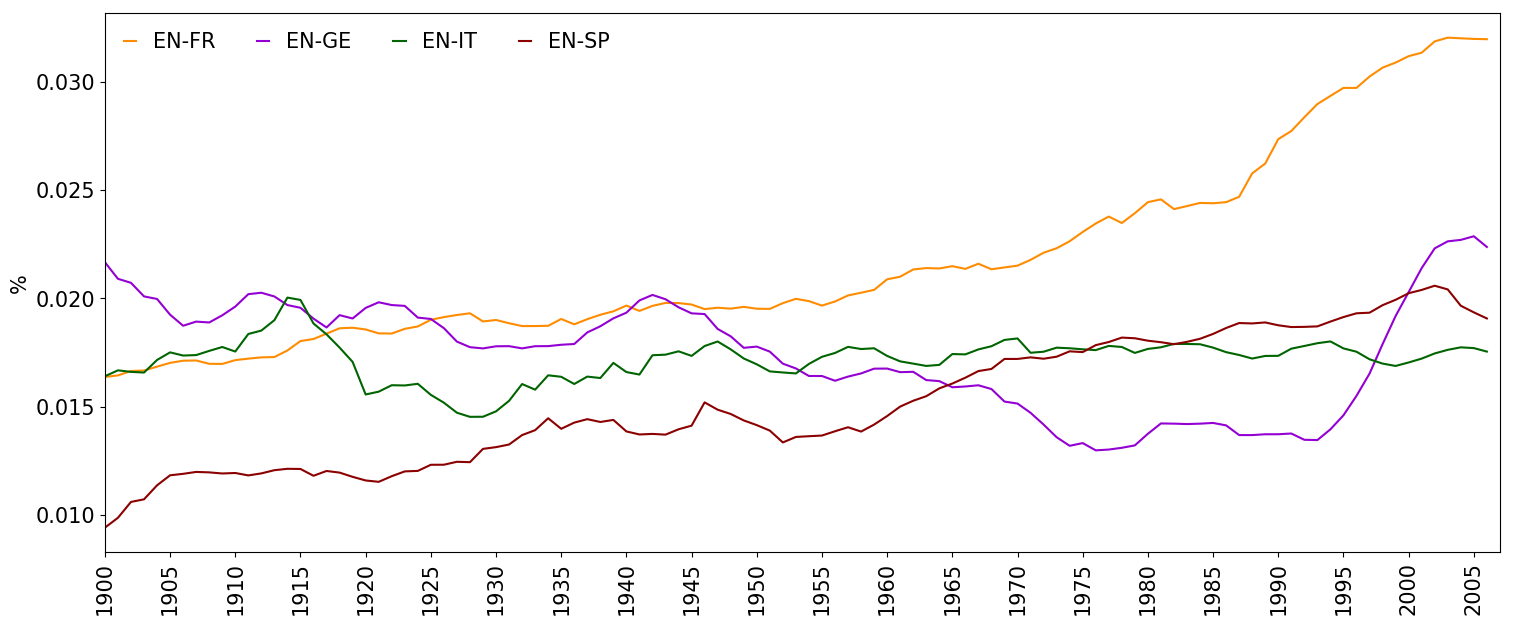
\includegraphics[scale=.36]{PF1_S2_EN.png}
	\label{fig.ST_a_EN}
	\caption{El inglés en los demás. El francés es el idioma donde más se ha empleado inglés, sin embargo en el español ha sido el de mayor crecimiento comparado en su uso en principios y en final de siglo.}
\end{figure} 



\begin{figure}[h!]
	\centering
	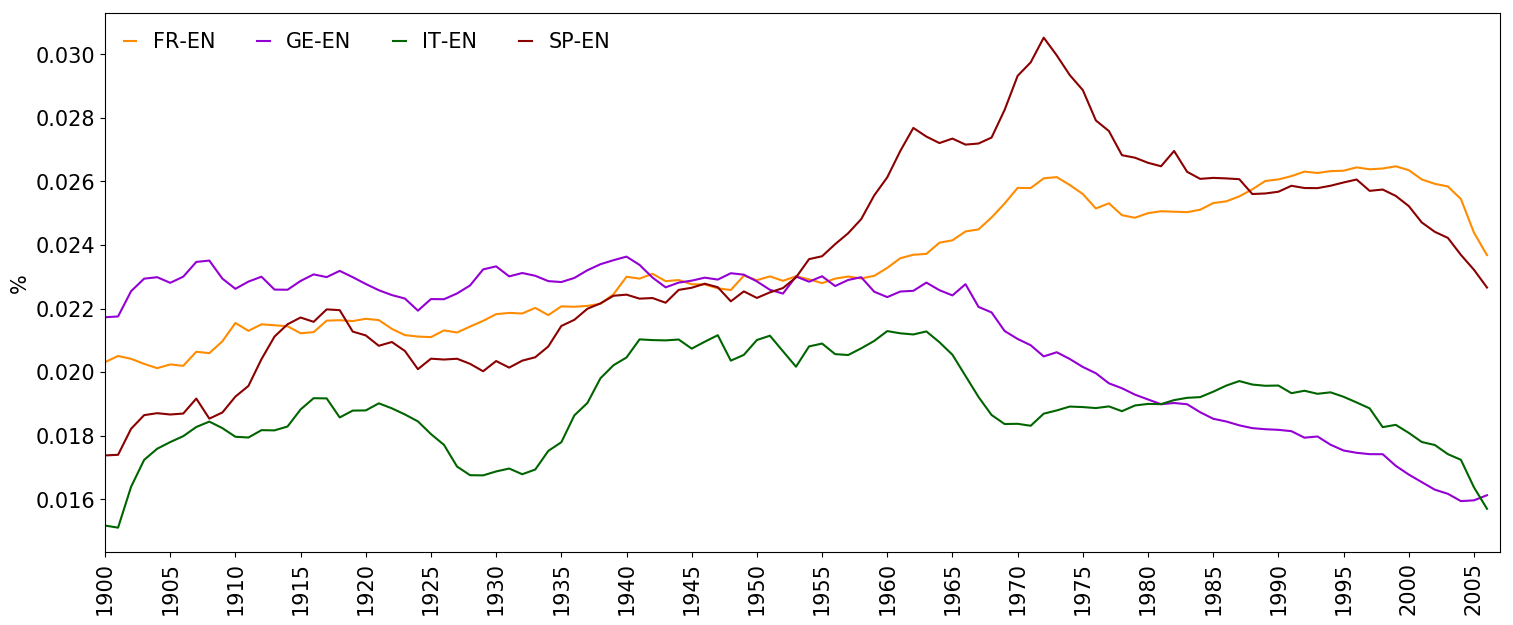
\includegraphics[scale=.36]{PF2_S2_EN.png}
	\label{fig.ST_b_EN}
	\caption{Los demás en el inglés. En los últimos 50 años, el español ha sido el idioma que es más utilizado en el ingles, seguido del francés, debido a las relaciones comerciales entre países de ambas lenguas.  Tras la segunda guerra mundial, alemán e italiano decayeron consistente en ser lengua de los países vencidos. }
\end{figure} 



El uso del ingles en los demás ha visto un continuo incremento posterior a 1945 en francés, en italiano y en español, mientras que en  alemán se da posterior a 1990, año donde culmina la guerra fría y se da la finalización del socialismo en Europa con la re-unificación de Alemania. El significado común de los   préstamos acumulados que aparecen en los cuatro conjuntos y que con los años descienden en rango son términos económicos y referentes a la industria como  \textit{capital}, \textit{dollar}, \textit{invesment}, \textit{relations}, \textit{market}, \textit{company}, \textit{development}, \textit{financial},  \textit{institutions}, \textit{internet} y \textit{software}. Otra característica relevante es la aparición continua de los apellidos de los presidentes de los Estados Unidos (posteriores a la guerra) durante el periodo en el cual gobernaron.  Apoyado de la información de los préstamos nuevos, se puede confirmar que el inglés se ha beneficiado del crecimiento de los Estados Unidos para ser exportado a las demás lenguas y ser el idioma común para transmitir información.   


En los últimos cincuenta años, los idiomas mas comunes en el ingles han sido el español y el francés,  nombres de países latinoamericanos como \textit{México}, \textit{Cuba}, \textit{Chile}, \textit{Nicaragua} y \textit{Argentina}, caracterizan a los acumulados del español, mientras que en el francés en su mayoría son palabras que bien podrian catalogarse de origen inglés, entre ellas \textit{royals}, \textit{religion}, \textit{saint}, \textit{passage} o \textit{court}. Tras brevemente ver ambos conjuntos se infiere que el español ha logrado instaurarse en el inglés por la relevancia de estos países en las relaciones o conflictos que tuvieron en el siglo pasado y donde intervinieron países de habla inglesa, contrario  al francés que prevalece por las relaciones culturales y etimológicas que existen entre ambas lenguas.

Por parte de las palabras con origen alemán e italiano no se logró relacionarlas a un campo semántico común. 


% }}}
\subsection{Francés} % {{{

\begin{figure}[h!]
	\centering
	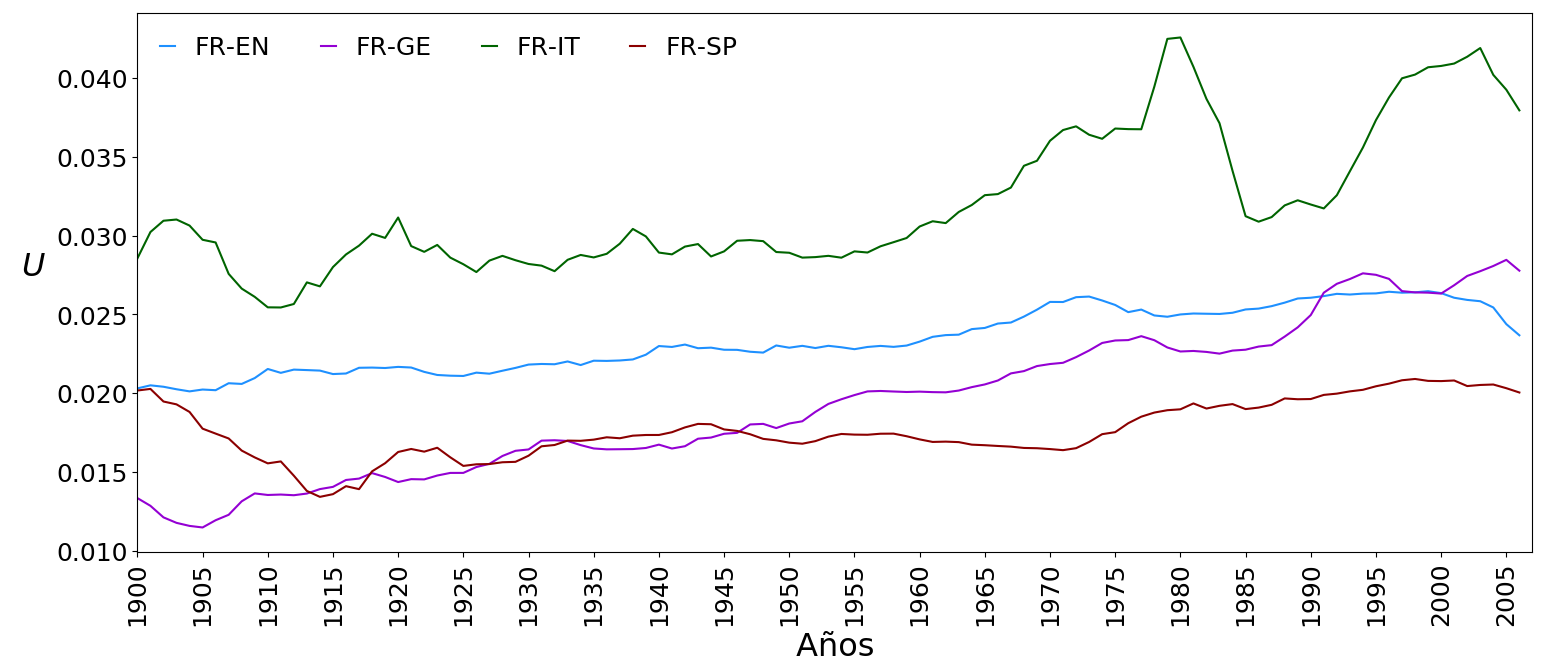
\includegraphics[scale=.36]{PF1_S2_FR.png}
	\label{fig.ST_a_FR}
	\caption{El francés en los demás idiomas. El italiano empleó más al francés durante todo el siglo XX, caracterizado por palabras comunes en la industria vitivinícola.}
\end{figure}


\begin{figure}[h!]
	\centering
	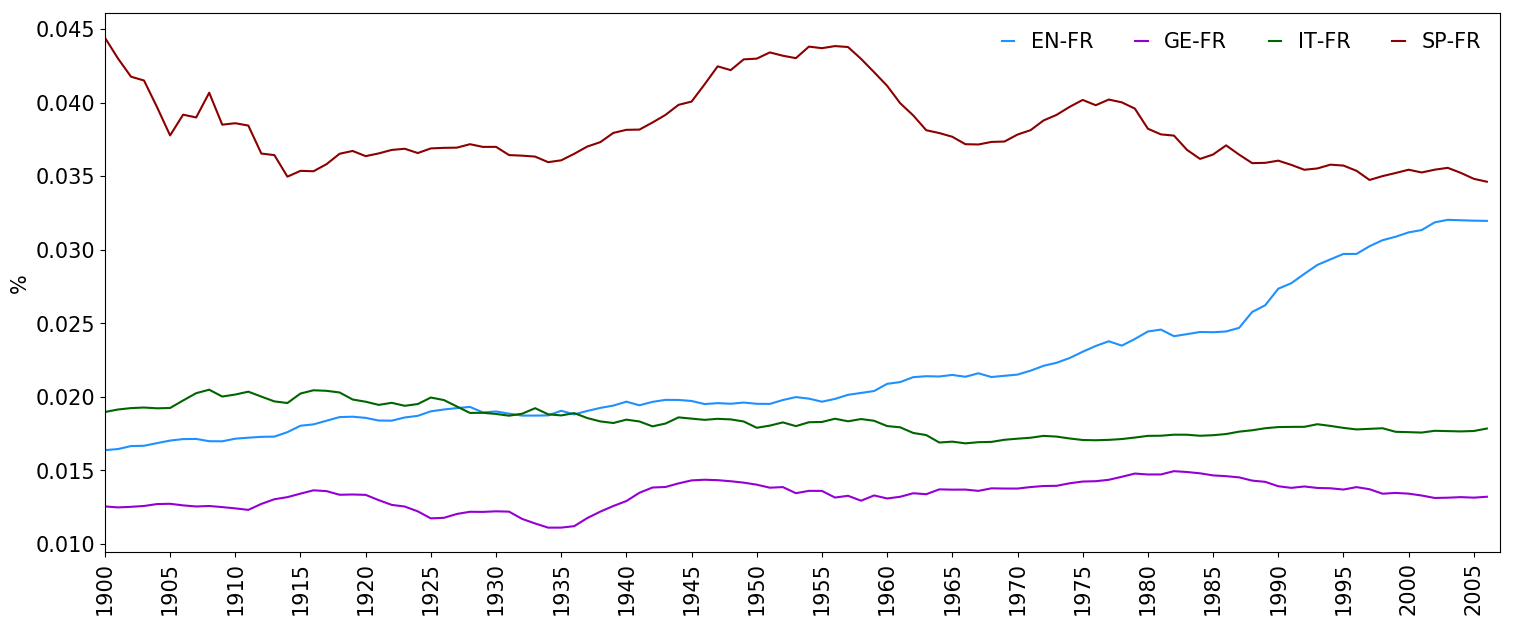
\includegraphics[scale=.36]{PF2_S2_FR.png}
	\label{fig.ST_b_FR}
	\caption{El español ha resultado el de mayor presencia en el francés, en su mayoria son palabras con etimologías grecolatinas, comunes para ambas lenguas al provenir de la misma familia lingüística.}
\end{figure}
		


A pesar de que el idioma que más préstamos toma del francés es el inglés,  el idioma que más utiliza el francés ha sido el italiano,  aspecto que se mantuvo durante todo el siglo del análisis,  la industria vitivinícola, surgen como un conectores entre ambas lenguas al estar presente términos como  \textit{raisins}, \textit{vin}, \textit{vignoble} y \textit{recolte},  siendo una actividad común entre Francia e Italia.  Los préstamos hacia los demás idiomas son de carácter religioso o politico, destacando que tuvo el francés en estos ámbitos, a pesar de que la búsqueda se centre en el siglo XX, las mayores migraciones del francés surgen a partir de 1800, posteriores a la revolución francesa; entre las palabras que se han mantenido desde este acontecimiento están  \textit{saint}, \textit{eglise}, \textit{dime}, \textit{reine}, \textit{guerre}, \textit{imperiale}, \textit{royals} o \textit{bourgeois}.  


Para los prestamos usados en el francés el español y el inglés se muestran como los idiomas con mayor presencia, la característica común de los vocablos de ambos idiomas es que son palabras con etimología grecolatina, 
\textit{depression}, \textit{canal}, \textit{proceso}, \textit{services}, \textit{justice} entre otras,  siendo razonable la aparición de estas palabras por tener las tres lenguas una composición grecolatina. 


% }}}
\subsection{Alemán} % {{{

\begin{figure}[h!]
	\centering
	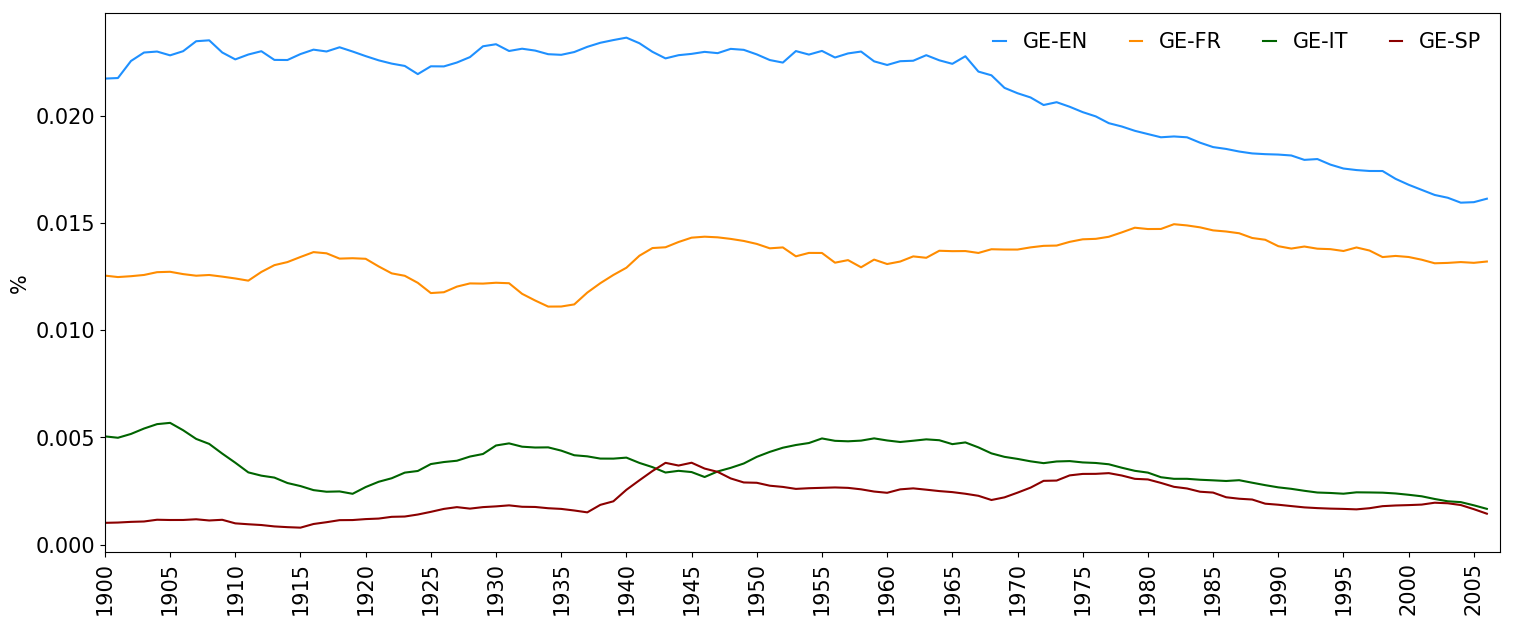
\includegraphics[scale=.36]{PF1_S2_GE.png}
	\label{fig.ST_a_GE}
	\caption{El alemán en los demás.}
\end{figure}


\begin{figure}[h!]
	\centering
	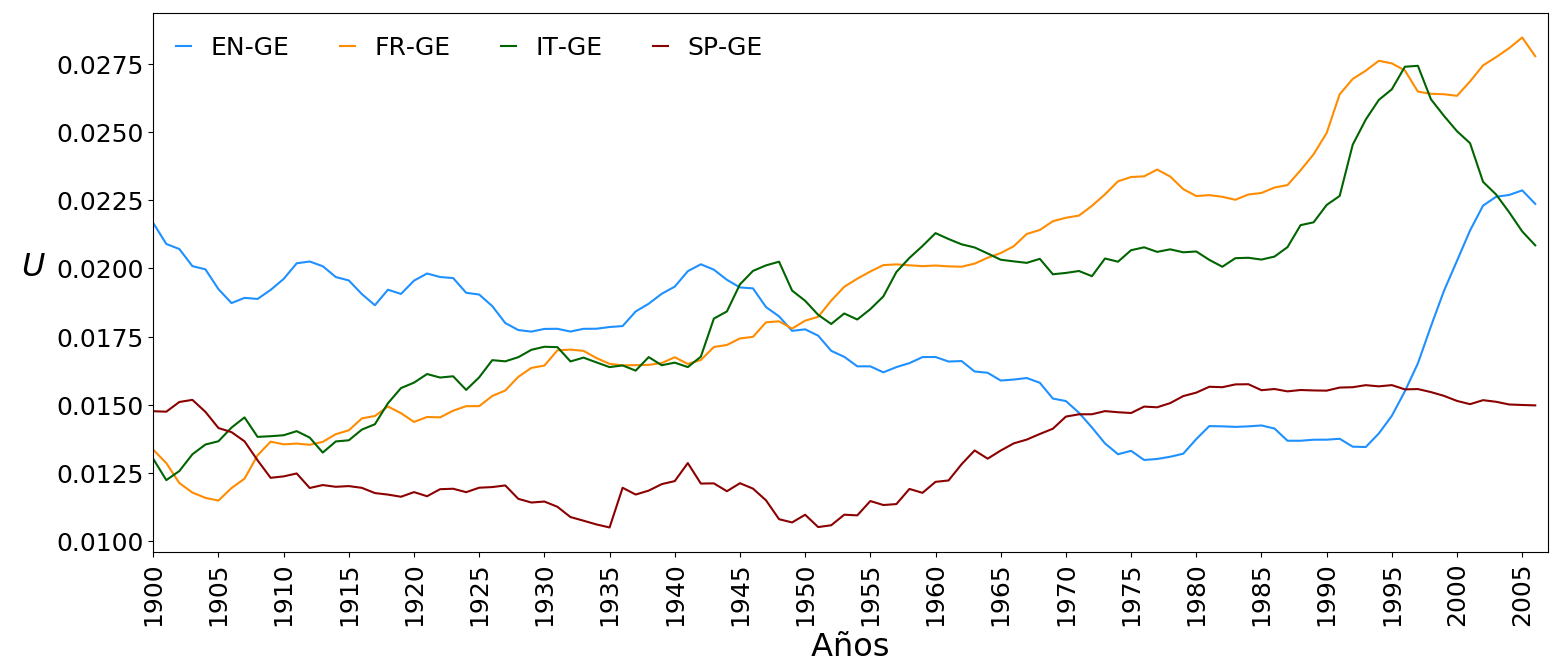
\includegraphics[scale=.36]{PF2_S2_GE.png}
	\label{fig.ST_b_GE}
	\caption{Los demás en el alemán}
\end{figure}



De acuerdo a la tabla \ref{table.PA},  el inglés, el francés, el italiano y el español, son en ese orden idiomas que más préstamos tienen provenientes del alemán, a pesar de que el alemán sea en cada uno el idioma del que menos se componen.  El orden de los idiomas que más emplean el alemán es el mismo que los idiomas que más se componen del alemán, siendo el único caso donde la mayor cantidad es también el mayor uso. Una razón de esta característica es que tanto el alemán como el inglés provienen de la misma familia lingüística, la germánica,  siendo más comunes las palabras entre ellos  que con las lenguas romances.

El sentido de cómo se utilizan los demás idiomas en el alemán, no presenta la característica anterior,   donde se ha alternado entre el inglés, el francés y el italiano el idioma que es más utilizado en el alemán.  El inglés fue el más empleado en la primera mitad del siglo, mientras que posterior a la guerra que ha sido el común detonante para que se altere el uso de un idioma en otro,  francés e italiano rolaron el papel del idioma más común en el alemán. 


% }}}
\subsection{Italiano} % {{{

\begin{figure}
	\centering
	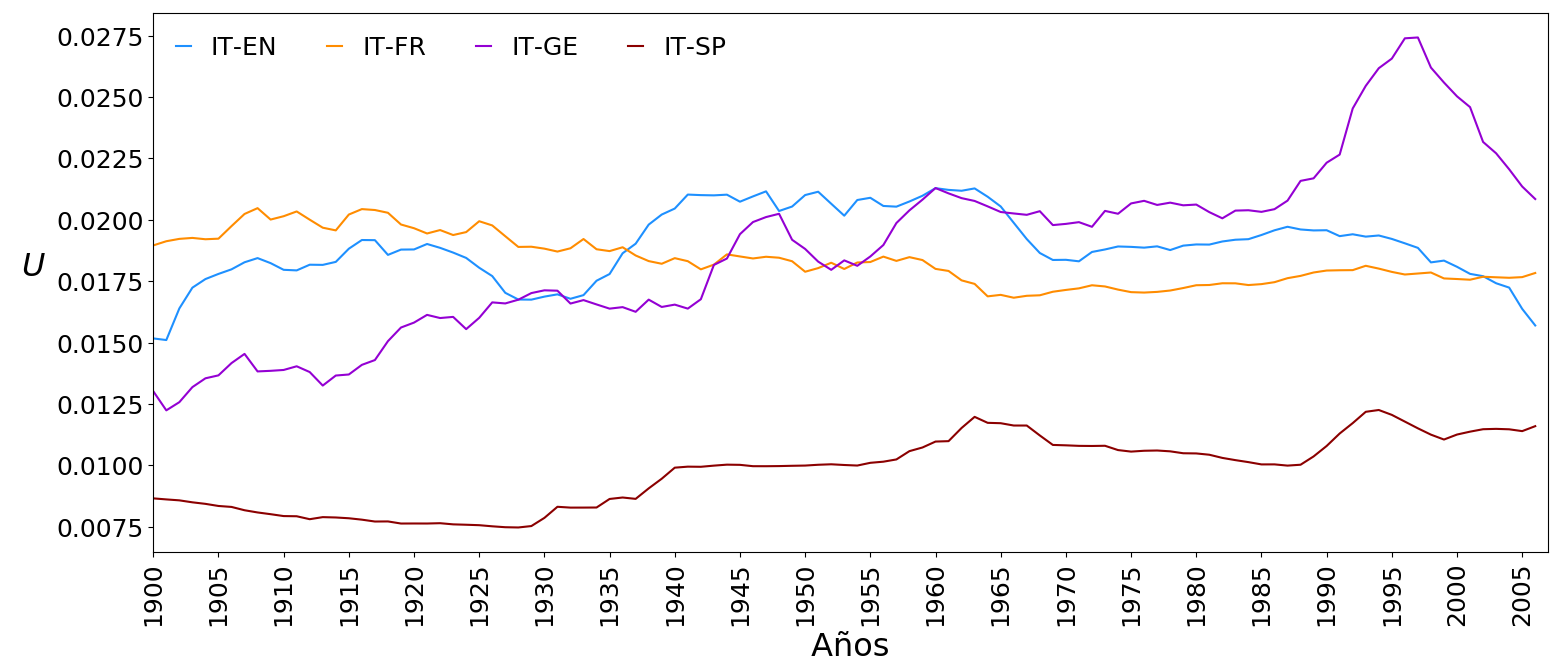
\includegraphics[scale=.36]{PF1_S2_IT.png}
	\label{fig.ST_a_IT}
	\caption{El italiano en los demás.}
\end{figure}
		
\begin{figure}[h!]
	\centering
	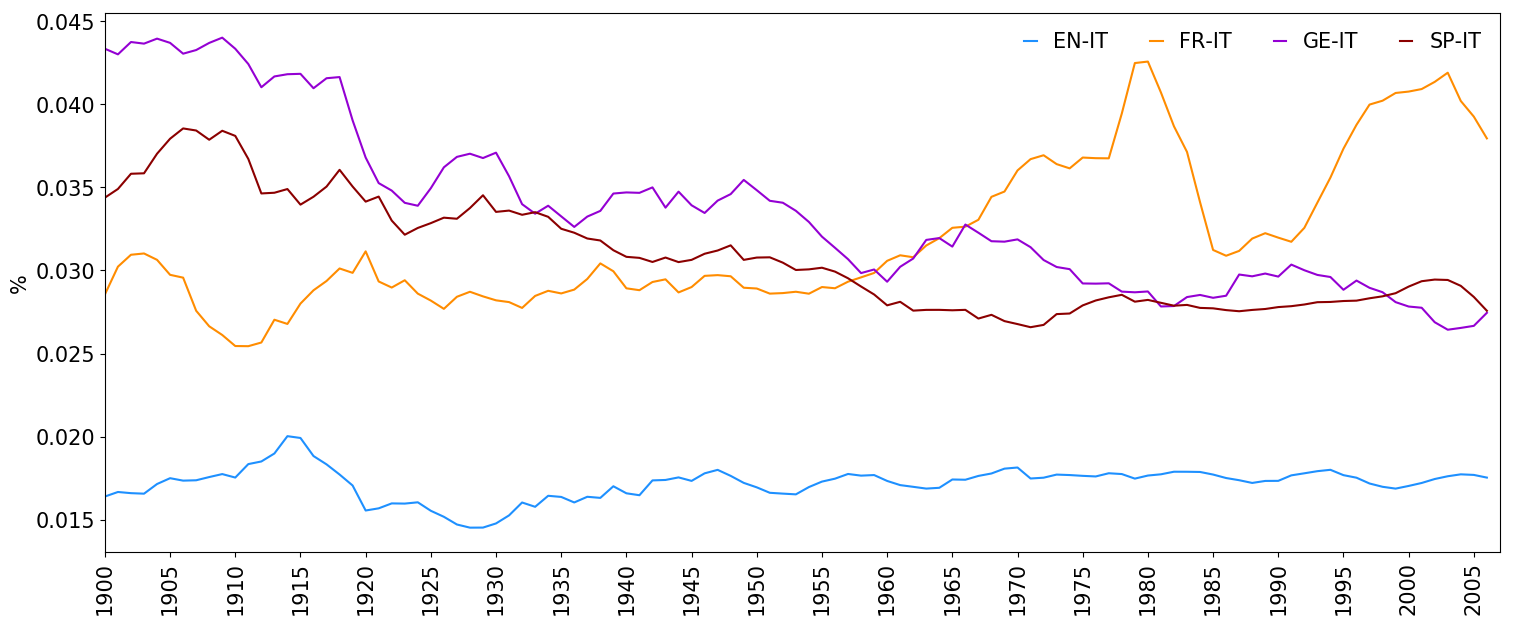
\includegraphics[scale=.36]{PF2_S2_IT.png}
	\label{fig.ST_b_IT}
	\caption{Los demás en el italiano.}
\end{figure}


Los idiomas en los que el italiano ha tenido una mayor influencia han sido el inglés, el francés y el alemán pese a que el español es el idioma que más préstamos contiene del  italiano,  circunstancias como la cercanía geográfica entre los países de habla alemán con Italia alude al  mayor uso del italiano en este idioma a partir de  la segunda mitad del siglo,  respecto al inglés,  la intervención de personajes  italianos en la historia y el hecho de que el inglés se compone de palabras de origen grecolatino,  permite que el italiano sea una lengua fuerte en el inglés;  las afirmaciones anteriores se han respaldado en que las palabras de contenido han sido previamente relacionadas  a sucesos donde han intervenido estos países.


La forma de actuar de los demás idiomas en el italiano no es recíproca a la forma en que el italiano interviene en ellos.  El caso del inglés es particular, porque a pesar del impacto que ha manifestado el inglés en los demás idiomas  en los últimos cincuenta años por la globalización,  en el italiano ha sido el único idioma donde no ha sido dominante en algún punto, o donde no ha crecido más que los demás.  El alemán ha sido más importante al comienzo del siglo y decae tras finalizar la segunda guerra mundial, para imponerse el francés como el idioma que más es utilizado en el italiano. 


% }}}
\subsection{Español} % {{{

\begin{figure}[h!] % {{{
	\centering
	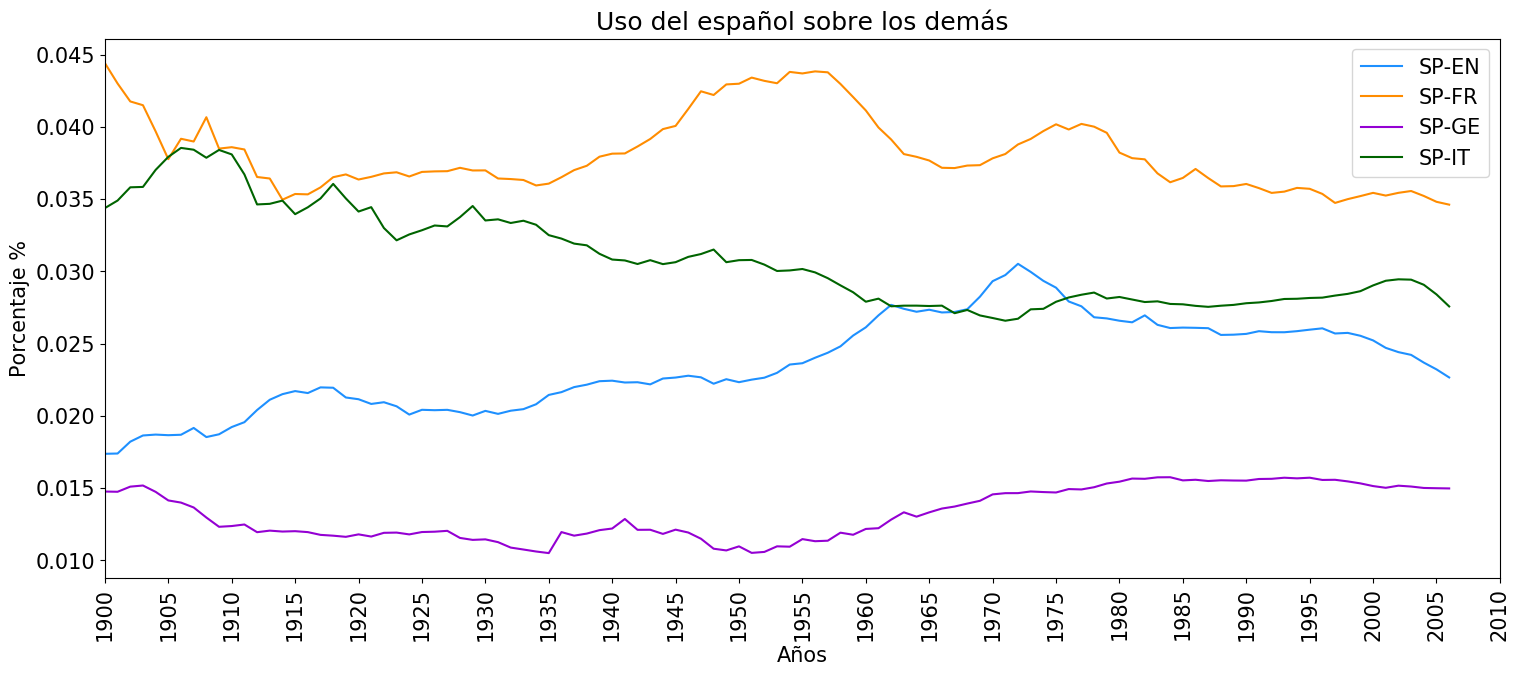
\includegraphics[scale=.36]{PF1_S2_SP.png}
	\label{fig.ST_a_SP}
	\caption{El español en los demás}
\end{figure} % }}}
		
\begin{figure}[h!] % {{{
	\centering
	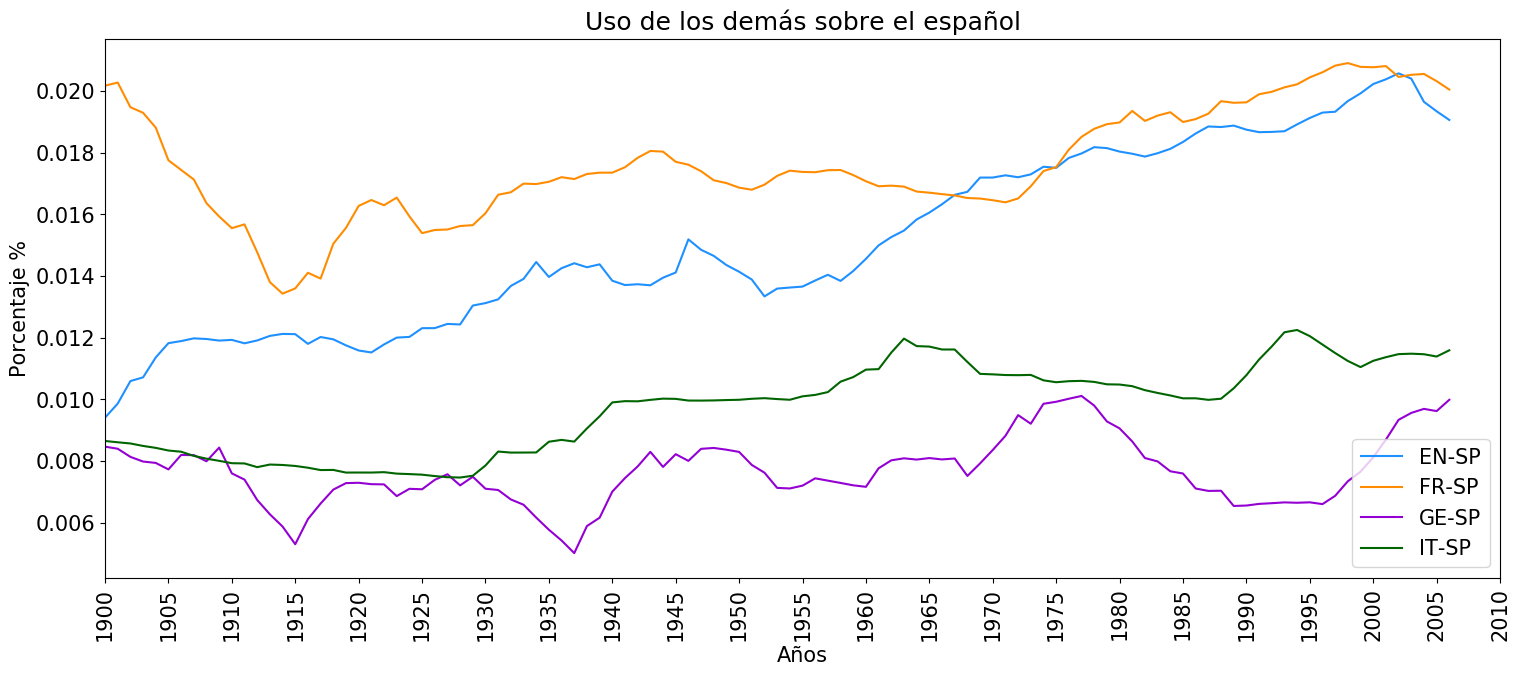
\includegraphics[scale=.36]{PF2_S2_SP.png}
	\label{fig.ST_b_SP}
	\caption{Los demás en el español.}
\end{figure} % }}}


Entre los gráficos del apéndice 1 de uso entre un determinado idioma y el español, se observó que el español ha sido más influyente en los demás que los demás en él,  siendo el francés el idioma donde el español es más utilizado, a pesar de que la cantidad de préstamos en el italiano es mayor, la causa mas lógica  de esta situación es el provenir ambos de la familia de las lenguas romances. 

Entre la forma en la que se usan los préstamos de los demás idiomas en el español,  en los últimos cincuenta años, la mayor influencia se ve compartida entre las palabras que vienen del francés y  del inglés;  la familia de las lenguas romances y sus similitudes hacen posible que el francés tome relevancia, mientras que la globalización y el crecimiento económico de países de habla inglesa hace relevante al inglés en el español.   Por otro lado,  el italiano y el alemán  no presentan el mismo crecimiento que el francés y el inglés,  por parte del italiano se ha comentado que al ser lengua romance al igual que el español,  el periodo donde los préstamos modificaban el uso del idioma receptor pudiese ser tan antiguo como el surgimiento de los idiomas,  por ello comparten gran cantidad de palabras pero estas no alteran el comportamiento del receptor; mientras que en el caso del alemán la poca relación con el español y el no haber existido un evento que los involucren,  hace que estos idiomas no se hayan mezclado como los demás,  por ejemplo alrededor de 1915 y 1935,  el alemán en el español es casi nulo, a pesar de que en esas fechas se desarrollaron las grandes guerras.

% }}}
% }}}
\section{Comentarios y complementos del método} % {{{


El determinar la influencia entre idiomas a través del uso de los préstamos, ha mostrado primeramente que el idioma que mas cantidad de palabras tiene en otro no siempre es el más utilizado,  radicando el mayor uso en aquel idioma cuyas préstamos tengan menores rangos en la lista de un receptor. 

En todo el siglo XX y la primer década del XXI, el inglés y el alemán han sido los idiomas más cambiantes en los papeles de origen y receptor respectivamente.
El inglés al ser el que más creció en tres idiomas (francés, alemán y español), complementando los resultados del capitulo anterior, al ser el idioma que más palabras nuevas exportó.  El alemán como el receptor donde los diferentes orígenes aumentaron su usó tras la segunda guerra mundial; el uso ha sido semejante a los préstamos nuevos, ha sido el receptor que más recibió. 

Ambos análisis se complementan,  el idioma más influyente ha aportado más palabras nuevas y aquellas que se van acumulando resultan las de mayor incremento en el uso. El idioma más influenciado recibió la mayor cantidad de palabras nuevas y el uso que han tenido los demás ha sido también el del mayor incremento. 

Por el momento sólo es posible describir que originó las variaciones en el uso o en la cantidad de nuevas palabras, no es posible predecir como se comportaran los idiomas en el futuro, ya que la principal característica que  hace fluir a las palabras entre idiomas han sido los eventos, reflejado en que las palabras de su campo semántico  se muevan a diferentes idiomas y continúen apareciendo o desapareciendo tras el suceso. 

Una mejor información de como los eventos alteran a los idiomas se podría extraer si se compararán las características de los prestamos con  datos de los países de alguna habla como lo pueden ser  el crecimiento economizo, el producto interno bruto, la alfabetización, la mortalidad, las migraciones de personas, entre otros.





% }}}

